% ---------------------------------------------------------------------------- %
\begin{figure}
  \centering
	\subfigure[\label{fig:results:mesh:complex:uovo}]
	{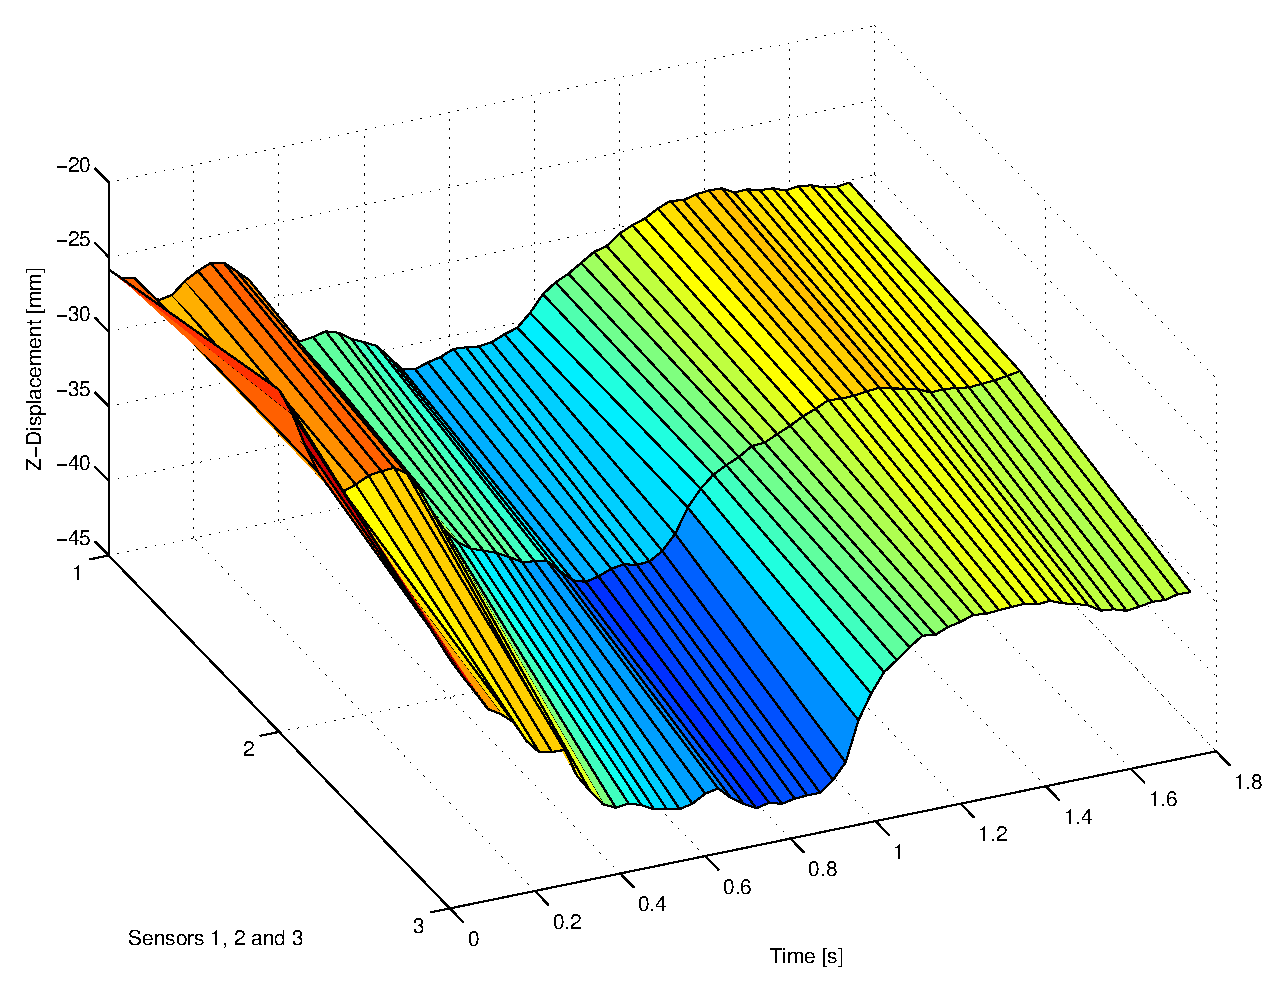
\includegraphics[width=0.45\textwidth]{include/results/images/complex_15_mesh.eps}}
	\hspace{0.05\textwidth}
	\subfigure[\label{fig:results:mesh:complex:giallo}]
	{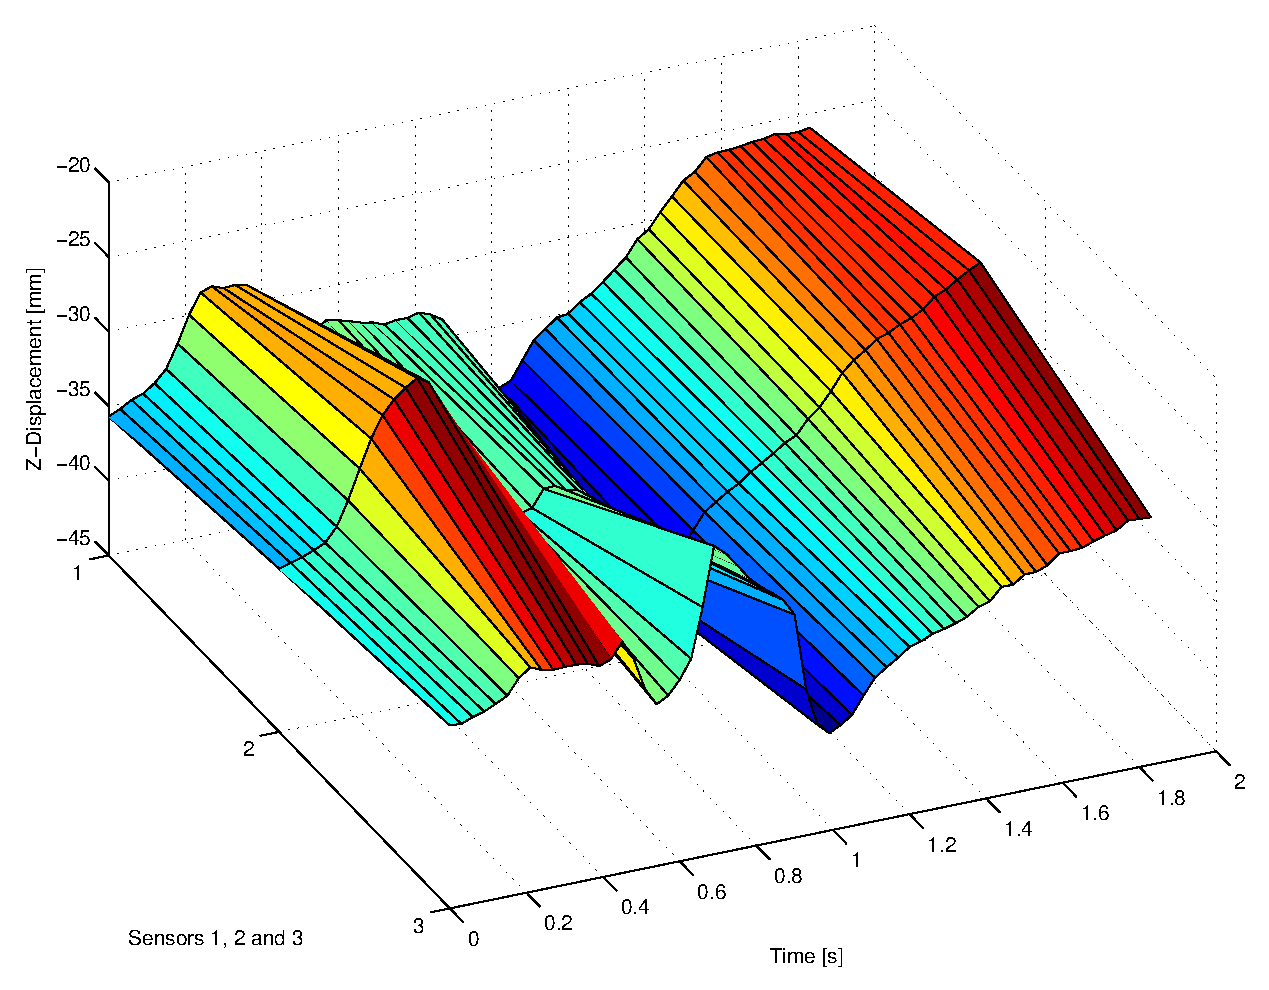
\includegraphics[width=0.45\textwidth]{include/results/images/complex_20_mesh.eps}}

	\caption[Vertical displacement of tongue for /uovo/ and /giallo/ (sagittal
	plane)]{\textbf{Vertical
	displacement of tongue for /uovo/ and /giallo/ (sagittal plane)}: 
	this plot provides a qualitative example for the vertical motion of the
	sensors glued sagittaly onto the tongue dorsum (sensors 1, 2 and 3).
	The kinesthetic information is acquired by the AG500 articulograph at
	a rate of 200 Hz. For the sake of simplicity, the data has been down-sampled
	by a factor of 6 before generating this plot (200 Hz / 6 = 33.3 Hz).
	}
	\label{fig:results:mesh:complex}
\end{figure}
% ---------------------------------------------------------------------------- %
